%%%%%This is a very basic article template.
%%%%%There is just one section and two subsections.
%%%\documentclass[11pt,a4paper]{article}
%%%
%%%\usepackage{graphicx}
%%%\usepackage{enumerate}
%%%\usepackage{listings}
%%%\lstset{language=[90]Fortran,
%%%  basicstyle=\ttfamily,
%%%  keywordstyle=\color{blue},
%%%  commentstyle=\color{green},
%%%  morecomment=[l]{!\ }% Comment only with space after !
%%%}
%%%\usepackage{amsmath,amssymb,amsfonts,mathrsfs,latexsym,cancel}
%%%\usepackage[total={16cm,25cm},top=2.5cm, right=2.5cm]{geometry}
%%%\usepackage{epstopdf}
%%%%Paquetes simbólicos:
%%%\newcommand{\dif}{\textrm{d}}
%%%\usepackage[utf8]{inputenc}
%%%\usepackage[spanish,es-nodecimaldot]{babel}
%%%
%%%\usepackage{lscape}
%%%\usepackage{array}
%%%
%%%\usepackage[usenames,dvipsnames]{pstricks}
%%% \usepackage{epsfig}
%%% \usepackage{epsf}
%%% \usepackage{float}
%%% \usepackage{pst-grad} % For gradients
%%% \usepackage{pst-plot} 
%%%
%%%\usepackage{float}%para que no ponga los graficos donde le de la gana, poner \begin{figure}[H]
%%%\usepackage{soul}%para poder remarcar texto, poner \hl{texto a subrayar}
%%%\usepackage[final]{pdfpages}
%%%%%%-- \includepdf[pages={x-y,{}(emptypages),x}
%%%\sloppy % suaviza les reglas de ruptura de l�neas de LaTeX
%%%\frenchspacing % usar espaciado normal despu�s de '.'
%%%
%%%\usepackage{babel}
%%%\usepackage{framed}
%%%\usepackage{mdframed}
%%%
%%%\newenvironment{blueframed}[1][blue]
%%%  {\def\FrameCommand{\fboxsep=\FrameSep\fcolorbox{#1}{white}}%
%%%    \MakeFramed {\advance\hsize-\width \FrameRestore}}
%%%  {\endMakeFramed}
%%%  
%%%\usepackage{relsize}
%%%
%%%\usepackage{blindtext} % provides blindtext with sectioning
%%%
%%%% \usepackage{scrpage2}  % header and footer for KOMA-Script
%%%% \pagestyle{scrheadings} 
%%%% %\thispagestyle{empty} %cuando una página la queramos sin encabezado
%%%% 
%%%% %headings---------------------------------------------------------------------------------
%%%% 
%%%% \rehead[]{\textit{Manual reference}}        % equal page, right position (inner) 
%%%% \lohead[]{\textit{Manual reference}}        % odd   page, left  position
%%%% % (inner)
%%%
%%%\usepackage{fancyhdr}
%%% 
%%%\pagestyle{fancy}
%%%\fancyhf{}
%%%\fancyhead[LE,RO]{\thepage}
%%%\fancyhead[RE,LO]{\textbf{Manual reference}}
%%% 
%%%\renewcommand{\headrulewidth}{0.5pt}
%%%
%%%
%%%
%%%%----------------------------------------------------------------------------------------------------
%%%
%%%\usepackage{appendix}
%%%\usepackage{multicol}
%%%\setlength{\columnsep}{7mm} %Espacio entre columnas en caso de hacer multicol
%%%\usepackage{xcolor}
%%%\usepackage{float}	
%%%\usepackage{subfigure}
%%%\usepackage[colorlinks=true,linkcolor=black]{hyperref}
%%%%\decimalpoint %Punto decimal en lugar de comma
%%%%Por si acaso:
%%%%\renewcommand{\contentsname}{Contenido}
%%%%\renewcommand{\partname}{Parte}
%%%%\renewcommand{\appendixname}{Ap�ndice}
%%%
%%%%\renewcommand{\abstractname}{Abstract}
%%%
%%%
%%%\usepackage{collectbox}
%%%\usepackage{tikz}
%%%\usepackage{forest}
%%%
%%%\usepackage{schemabloc}
%%%\usepackage{pst-tree,array}  
%%%
%%%\makeatletter
%%%\newcommand{\sqbox}{%
%%%    \collectbox{%
%%%        \@tempdima=\dimexpr\width-\totalheight\relax
%%%        \ifdim\@tempdima<\z@
%%%            \fbox{\hbox{\hspace{-.5\@tempdima}\BOXCONTENT\hspace{-.5\@tempdima}}}%
%%%        \else
%%%            \ht\collectedbox=\dimexpr\ht\collectedbox+.5\@tempdima\relax
%%%            \dp\collectedbox=\dimexpr\dp\collectedbox+.5\@tempdima\relax
%%%            \fbox{\BOXCONTENT}%
%%%        \fi
%%%    }%
%%%}
%%%\makeatother
%%%
%%%
%%%\usepackage{graphicx}% just for the example text
%%%
%%%
%%%%Otros paquetes:
%%%%\pagestyle{empty} %Eliminar numeraci�n p�gs
%%%%\parskip=Xmm %Espacio entre p�rrafos
%%%%\headheight %Altura cabecera
%%%\parindent=0mm %Eliminar sangr�a
%%%%\pagestyle{myheadings}: Coloca la numeraci�n de p�gina en la parte superior
%%%%\markright{�texto�}: Coloca �texto� en la parte superior de la p�gina. Se pueden
%%%%poner varios \markright en el texto (en cada secci�n, por ejemplo).
%%%%\newpage: Le indica a LATEX que siga imprimiendo en la p�gina siguiente
%%%\newtheorem{Teorema}{Teorema}
%%%\title{\textbf{Manual reference}}
%%%\author{Pablo L\'opez Negro}
%%%%=============================================================================
%%\begin{document}

%%%=============================================================================
%%%===========================Language===================================
%%\renewcommand{\figurename}{Figure}
%%\renewcommand{\tablename}{Table}
%%\renewcommand{\refname}{References}
%%\renewcommand{\contentsname}{Table of contents}
%%\renewcommand{\listfigurename}{List of figures}
%%\renewcommand{\listtablename}{List of tables}
%%\renewcommand{\appendixname}{Appendix}
%%\renewcommand{\appendixtocname}{Appendix}
%%\renewcommand{\appendixpagename}{Appendix}
%%%=============================================================================
%%%============================PORTADA===========================================
%%
%%%\includepdf[pages=1]{cover}
%%
%%
%%
%%%============================ABSTRACT==========================================
%%% \newpage
%%
%%%\includepdf[pages=1]{abstract}
%%
%%%============================INDEX============================================
%%\newpage
%%\thispagestyle{empty}
%%
%%{\huge{\underline{Manual reference}}}\\\\
%%
%%{\Large{\textbf{High-order finite differences library}}}\\
%%
%%{\large{\textbf{Application programming interface}}}
%%
%%{\begin{centering}
%%\rule {16cm}{1pt}
%%\end{centering}}
%%
%%\vspace{1cm}
%%



The aim of this paper is to present a brief description of a library
prepared to execute the \wk{spatial discretization} of any given function. \\

This library is written in Fortran programming language, and holds all the
operations needed in order to perform the spatial discretization of a function
using high order interpolation and \wk{finite differences} schemes. \\

This document is focused in explaining the \underline{application programming
interface} of the library. \\

A precise description of the internal procedures is beyond the purpose of this paper. 
The idea is to present the essential information in order to
understand and \textbf{\underline{use}} the software. 

\newpage

\section{Introduction}

When solving a \ww{PDE problem}, \index{PDE problem- partial derivative equation
problem} some operations for the spatial discretization of the function are
performed. This module contains the operations and procedures needed in order to discretize, interpolate and derive a function. \\

This library holds all the procedures needed for this purpose. However, its
functionality goes further from this application: it can be used for the whole
spatial discretization, or just to solve the derivative of a function. \\

The following box holds the operations that the library can accomplish and the
subroutine which performs the action.\\

\begin{framed}
{\Large{\textbf {High Order Finite Difference Library}}}\\

\begin{multicols}{2}

\begin{framed}
{\large{\textbf{Grids}}}\\

\hspace{0.5cm} Grid \hfill \framebox[3cm]{Grid initialization}\\
\vspace{1.12cm}

\end{framed}

\begin{centering}

\begin{Huge}
$\Updownarrow$
\end{Huge}

\end{centering}

\columnbreak

\begin{framed}
{\large{\textbf{Finite differences}}}\\

\hspace{0.5cm} Derivatives \hfill \framebox[3cm]{Derivatives}\\

\hspace{0.5cm} Boundary conditions \hfill $\begin{cases}
\boxed{Dirichlet}\\ \boxed{Newmann}
\end{cases}$\\

\end{framed}

\begin{centering}

\begin{Huge}
$\Updownarrow$
\end{Huge}

\end{centering}

\end{multicols}


\begin{framed}

\begin{centering}

{{\textbf{Lagrange interpolation}}}

\end{centering}

\end{framed}



\end{framed}

% \begin{framed}
% {\Large{Plotting Library}}\\
% 
% \hspace{2cm}Results, outputs and graphs \hfill $\Longrightarrow$ 
% \framebox[5cm]{Dislin}\\
% 
% \end{framed}


\vspace{0.5cm}

The following sections will describe the sentences and the syntax of each
operation in order to use the library. The collection of function calls will
configure the \wk{API} of this library.\\

Finally, some examples are presented for fixing ideas. \\

\newpage

\section{Meshing}

\wb{Grid\_Initialization}

This routine will calculate a set of points within the space domain defined;
$[-1,1]$ by default.

\begin{blueframed}
\begin{lstlisting}
call Grid_Initialization( "grid_type", direction, Order, x )
\end{lstlisting}
\end{blueframed}

\begin{itemize}
  \item {\textit{grid\_type}: here the \wk{grid} structure must be chosen. It
  can be 'uniform' (equally-spaced) or 'nonuniform'. }
  \item {\textit{direction}: 'x', 'y' or 'z'.}
  \item {\textit{order}: this is the order chosen for the \wk{interpolating
  polynomials}. This label is for the software to be sure that the number of
  nodes ($N$) is greater than the polynomials order (at least $N= order +1$).
  %(\underline{Otherwise an error message will appear}.)  
  }
  \item {\textit{x}: vector containing the \wk{mesh} nodes.}
\end{itemize}

This is important to remark that this function is very powerful: let's imagine a
2D problem. The mesh will be created just with two calls with the same syntax: 

\begin{blueframed}
\begin{lstlisting}
call Grid_Initialization( "uniform", "x", Order, x )
call Grid_Initialization( "nonuniform", "y", Order, y )
\end{lstlisting}
\end{blueframed}

Also, the example shows how different meshes can be chosen along each direction.
\\

\vspace{1cm}

\section{Numerical differentiation}

\wb{Derivative}

The library uses \wk{finite differences} to approximate the derivatives of the
function. This routine is called with the following sentence: 

\begin{blueframed}
\begin{lstlisting}
call Derivative( "Direction", k, U, Uxk) 
\end{lstlisting}
\end{blueframed}

This call performs the operation: $\frac{\delta^k U}{\delta x^k}=U_{xk}$.\\

Generally speaking, the arguments of the function are: 

\begin{itemize}
  \item \textit{Direction}.
  \item \textit{Derivative order} (first derivative, $k=1$; second derivative,
  $k=2$ and so on).
  \item \textit{Function values}. 
  \item \textit{Result}: (output)- the $k$-derivative of the given function. 
\end{itemize}

The routine is prepared to be called equally in 1D, 2D and 3D problems. The
difference is inside the $U$ array structure: if $U$ has the shape $U(:)$ the
routine assigns the 1D procedures for differentiation, while, if $U(:,:)$, the
routine will continue with 2D operations.\\

\subsection*{Example. Laplacian of a function}

The calculation of the \wk{Laplacian}, operation that might be hard to code from
the beginning, is now very easy using the library. Let's assume we have the
function $U=f(x,y)$ evaluated in a set of points and allocated in an
array of the shape $U(0:N_x, 0:N_y)$. Then, the laplacian is easily
calculated: \\



\begin{blueframed}
\begin{lstlisting}
	call Derivative( "x", 2, U, Uxx) 
	call Derivative( "y", 2, U, Uyy) 

	L=Uxx+Uyy
\end{lstlisting}
\end{blueframed}

With these commands, an array $L(:,:)$ is obtained, containing the value of the
laplacian of the function in the points of the discretization. Go to section
\ref{laplacian} to find the complete example code.\\


\section{Boundary conditions}

When dealing with a \ww{PDE problem}, the \wk{boundary conditions, BC,} should
be discretized as well. Sometimes the BC can be as complex as the main equations, however,
there are some common conditions that can be written in an universal notation,
so the library can solve them. \\

For now, we have to choose the boundary conditions between \wb{Neumann} and
\wb{Dirichlet} since more arbitrary functions have not been included in the
library. \\



% % The purpose is to develop a routine able to solve arbitrary conditions;
% % something like: 
% % 
% % \begin{framed}
% % \begin{lstlisting}
% % call Boundary_conditions( "BC_type", "direction", point, U, f)
% % \end{lstlisting}
% % \end{framed}
% % 
% % Where we must define: 
% % \begin{itemize}
% %   \item {\textit{Boundary condition}: 'Dirichlet', 'Neumann' \ldots
% %   \footnote{Also, it will be interesting to add the possibility of calling a 'user defined'
% %   function for solving an arbitrary condition. This is not implemented yet.}}
% %   \item {\textit{Direction}: 'x', 'y', 'z'. }
% %   \item {\textit{Point}: point index where the condition is
% %   applied.\footnote{For example, $point=N_x$ will assign the boundary condition to $x(N_x)$.} }
% %   \item {\textit{Function value}: this is an in/out array containing the
% %   function values in all the mesh' points. $U$ can be $U(:)$,
% %   $U(:,:)$ and $U(:,:,:)$, depending on the problem dimension.}
% %   \item {\textit{Boundary condition value}, f; which could be a time dependent.}
% % \end{itemize}
% % 
% % Unfortunately this is not implemented yet. 

\subsection{Boundary condition type 'Dirichlet'}

A BC type \wb{Dirichlet} is defined as: 
$$
  		\mathbf U(\mathbf x_0, t)= \mathbf f(\mathbf x_0,y_0,t) \hspace{1cm} 
  		\mathbf{x_0} \in \delta \Omega \\
$$

And the routine should be called as follows: 

\begin{blueframed}
\begin{lstlisting}
call Dirichlet( "direction", N, U, f ) 
\end{lstlisting}
\end{blueframed}

With the syntax that has already been described. \\

The routine takes the array $U$ and substitutes the element $N$ by the value of
$f$. For example:

\begin{blueframed}
\begin{lstlisting}
call Dirichlet( "x", N_x, U, f_1 ) 
call Dirichlet( "y", N_x, U, f_2 ) 
\end{lstlisting}
\end{blueframed}

These statements perform the following operations: 

$$
U(N_x,:)=f_1; \hspace{1cm}
U(:,N_y)=f_2
$$

\subsection{Boundary condition type 'Neumann'}

This BC is a bit more complex: 
$$
\frac{d \mathbf U}{d \mathbf n}(\mathbf{x_0},t)= \mathbf f(\mathbf{x_0},t)
  		\hspace{1cm}  \mathbf{x_0}
  		\in \delta \Omega 
  		$$

However, the power of this library is that this complexity is encapsulated
inside internal procedures, and, from the API, all that is needed is the usual assignment: 

\begin{blueframed}
\begin{lstlisting}
call Newmann( "direction", N, U, f ) 
\end{lstlisting}
\end{blueframed}

For 1D problems, the argument \textit{direction} must not be written.\\

\newpage

\section{Examples}

Briefly, the purpose of this paper is just to give a general perspective about
how to work with the \wk{high-order finite difference} library. The following
pages present a set of examples which may be interesting and helpful in order to
practise the ideas of this text. \\

After this brief presentation of the methods, one should be able to perform the
\wk{spatial discretization} of any given problem.\\


%============================APPENDIX========================================

% \appendix
% % \addcontentsline{toc}{section}{Appendices}


\subsection{ Derivatives 1D}

This example calculates the first and second \wk{derivative} of the function
$U=sin(\pi x)$. \\

\begin{blueframed}
\begin{lstlisting}
program Example

	use Finite_differences
	use dislin   			!for plotting results
	implicit none
	
  	integer, parameter :: N= 50;!number of points
  	real ::  x(0:N)
	real:: U(0:N)
	real:: Ux(0:N), Uxx(0:N)
	integer :: Order = 20	!order of the interpolation
	real :: pi = 4*atan(1.) 

	call Grid_Initialization( "uniform", "x", Order, x )
	
	!function U=f(x)
	
	U=sin(pi*x)
	
	call Derivative( "x", 1, U, Ux) 
	call Derivative( "x", 2, U, Uxx) 


	! Outputs (optional)
	call scrmod('revers') 
	call qplot(x, U, N+1)
	call qplot(x, Ux, N+1)
	call qplot(x, Uxx, N+1)

end program
\end{lstlisting}
\end{blueframed}

\newpage
\begin{landscape}
\subsubsection*{ Results }

The following figures present the results obtained using the numerical procedure
described above. Results for \ww{uniform and non uniform meshes} (first line
vs. second line of figures, respectively), 10 (o), 20 points (+) and exact
solution (dashed line).

\begin{multicols}{3}

\begin{figure}[H]
\centering
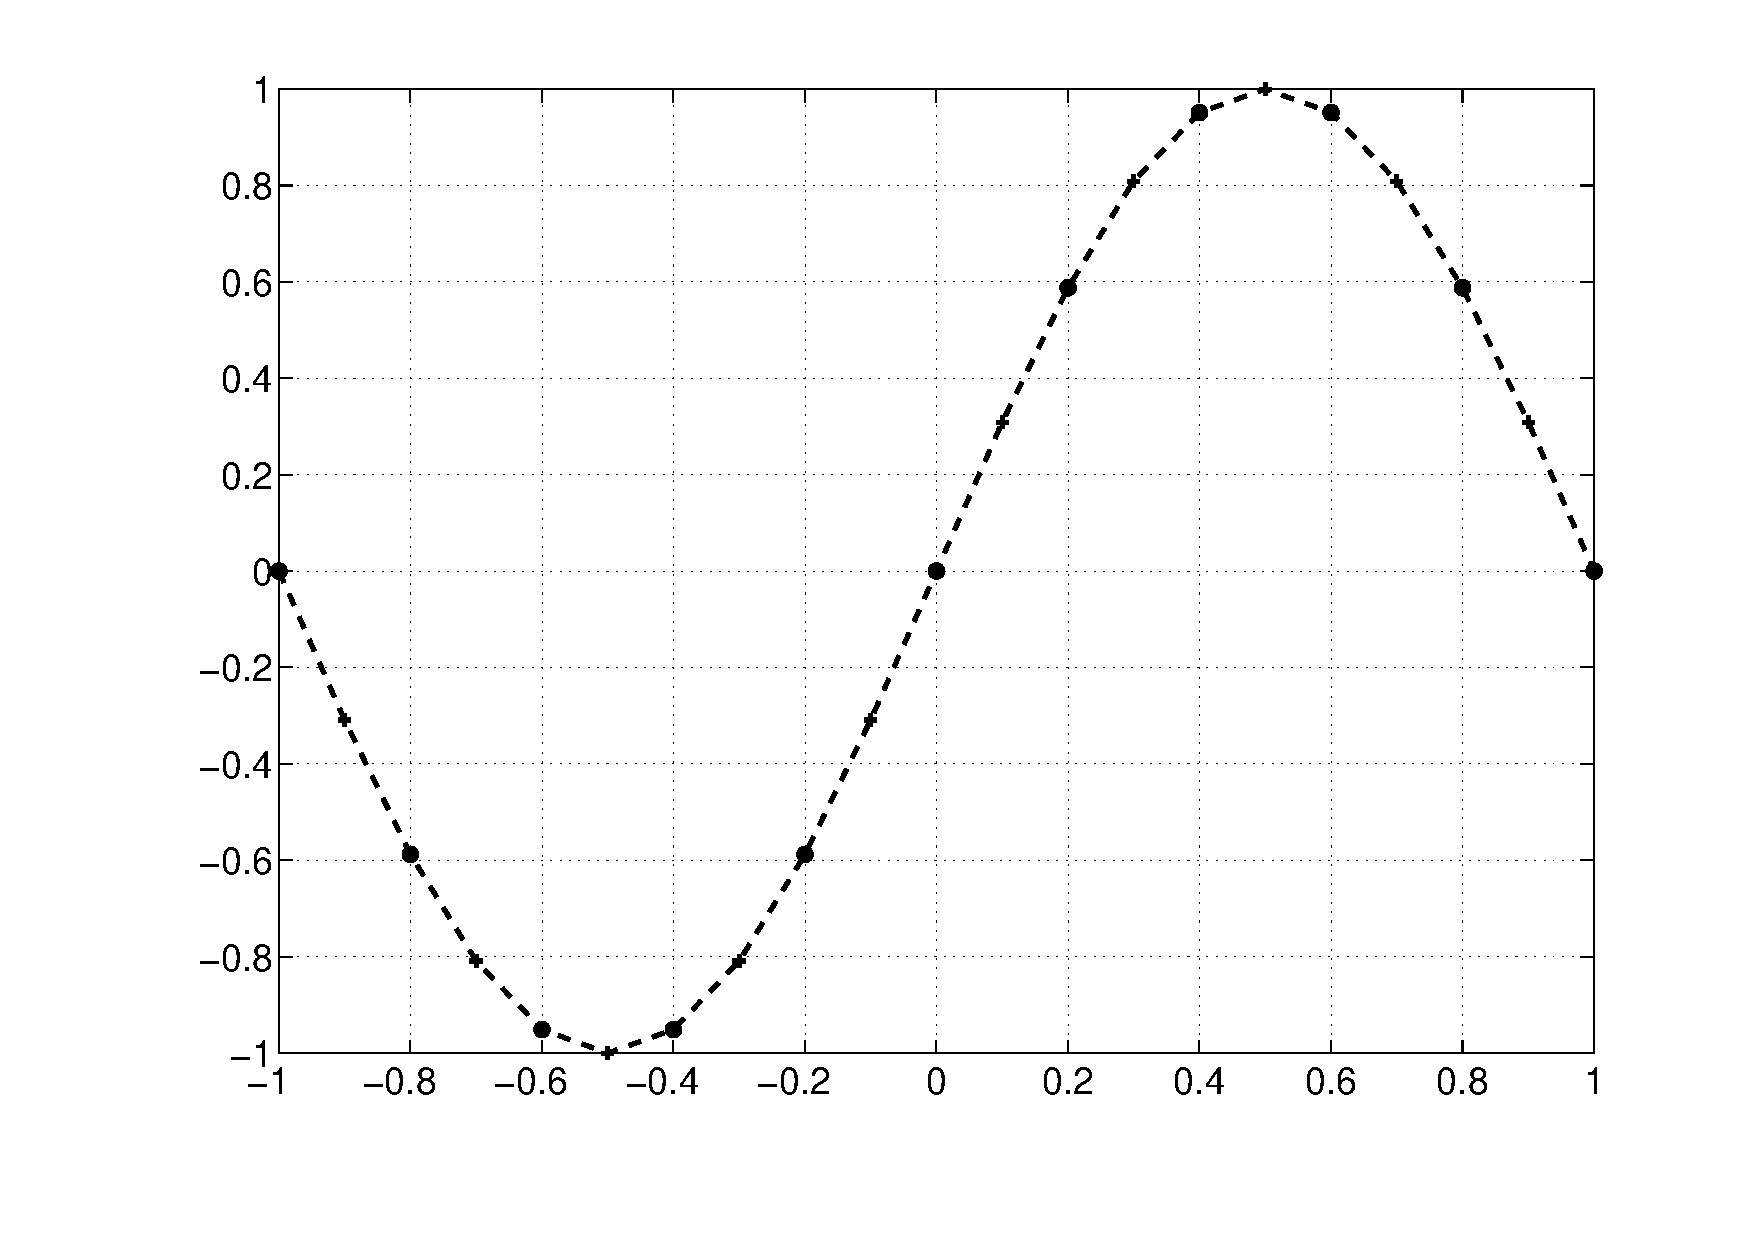
\includegraphics[scale=0.3, trim = 20mm 0mm 0mm 0mm, clip]{./Figures/1-HOFD/u_u.pdf}
\caption{$f(x)= sin(\pi x)$, uniform mesh. }
\end{figure}

\columnbreak

\begin{figure}[H]
\centering
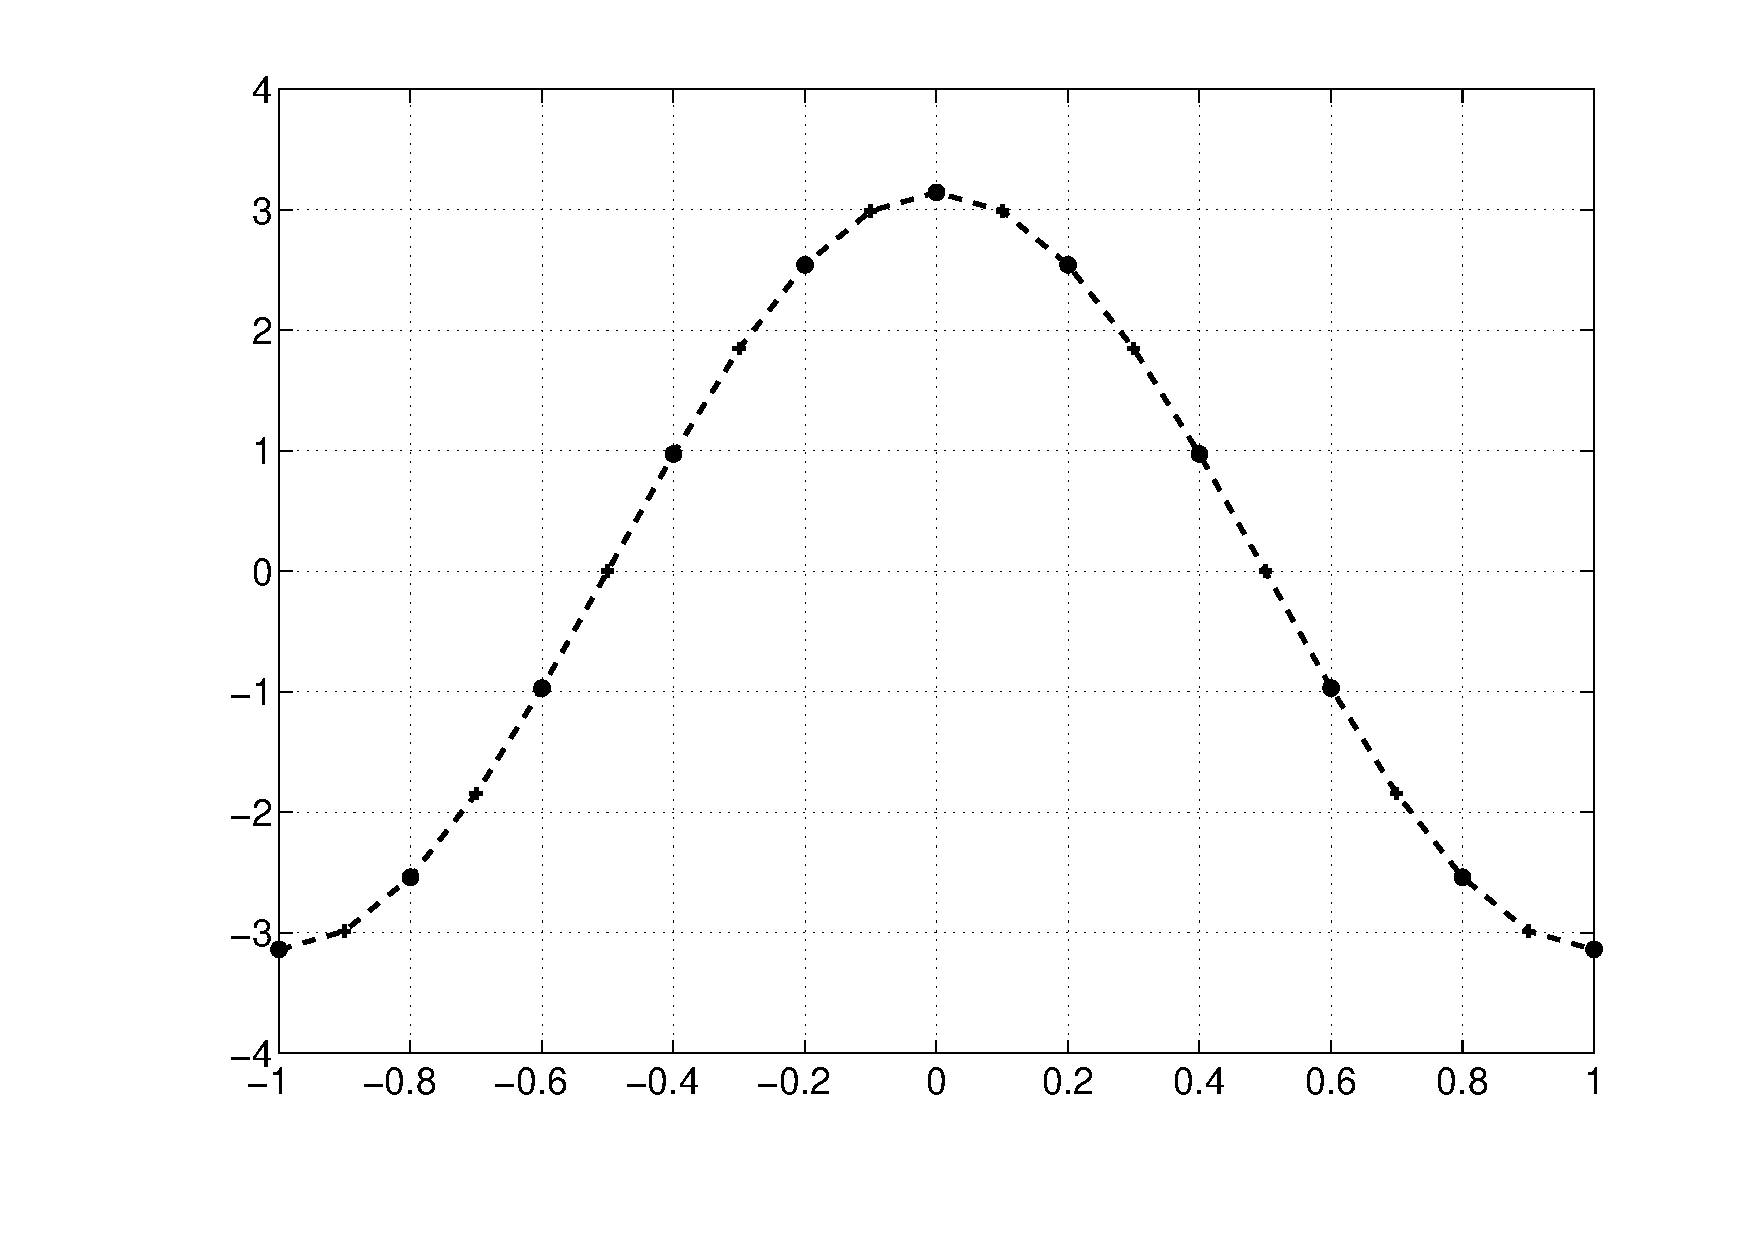
\includegraphics[scale=0.3, trim = 20mm 0mm 0mm 0mm, clip]{./Figures/1-HOFD/du_u.pdf}
\caption{$f'(x)$, uniform mesh. }
\end{figure}

\columnbreak

\begin{figure}[H]
\centering
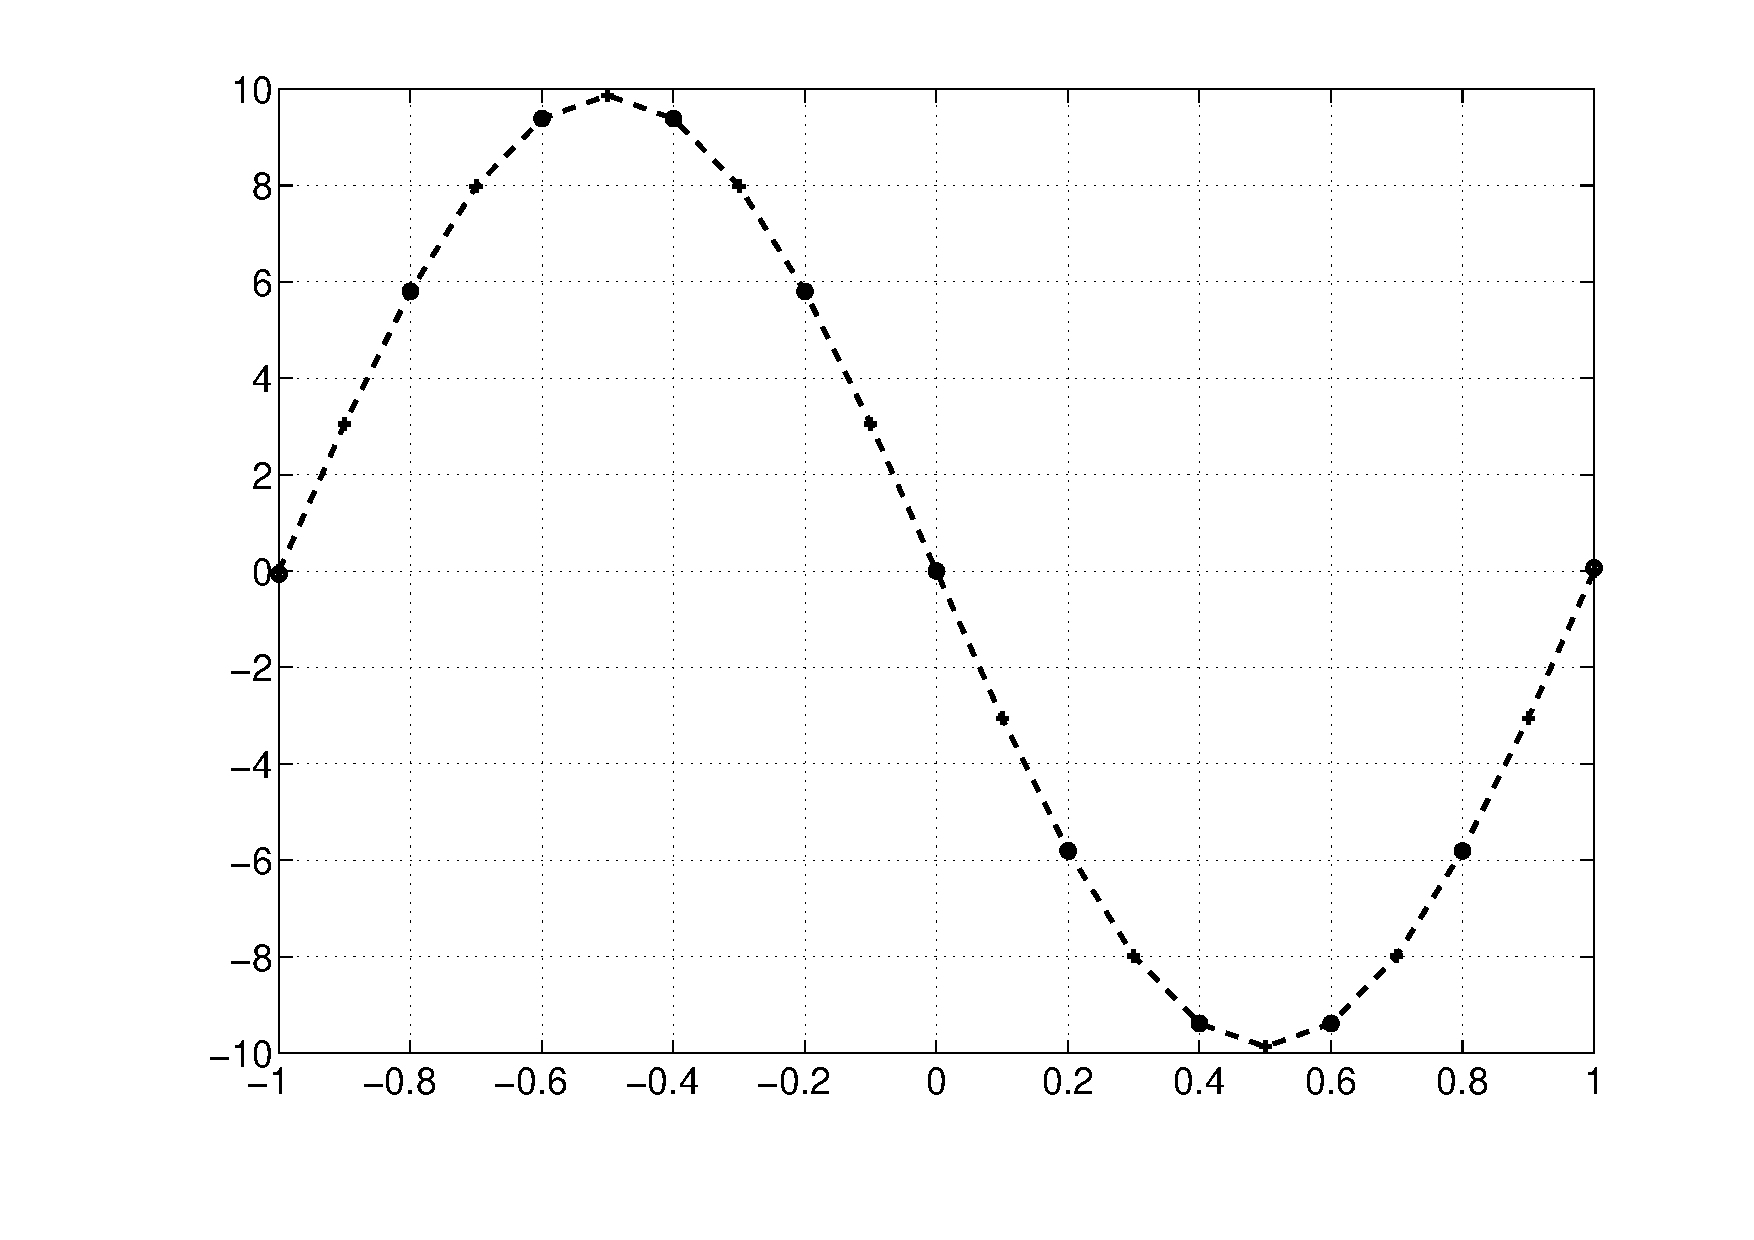
\includegraphics[scale=0.3, trim = 20mm 0mm 0mm 0mm, clip]{./Figures/1-HOFD/ddu_u.pdf}
\caption{$f''(x)$, uniform mesh. }
\end{figure}

\end{multicols}

\begin{multicols}{3}

\begin{figure}[H]
\centering
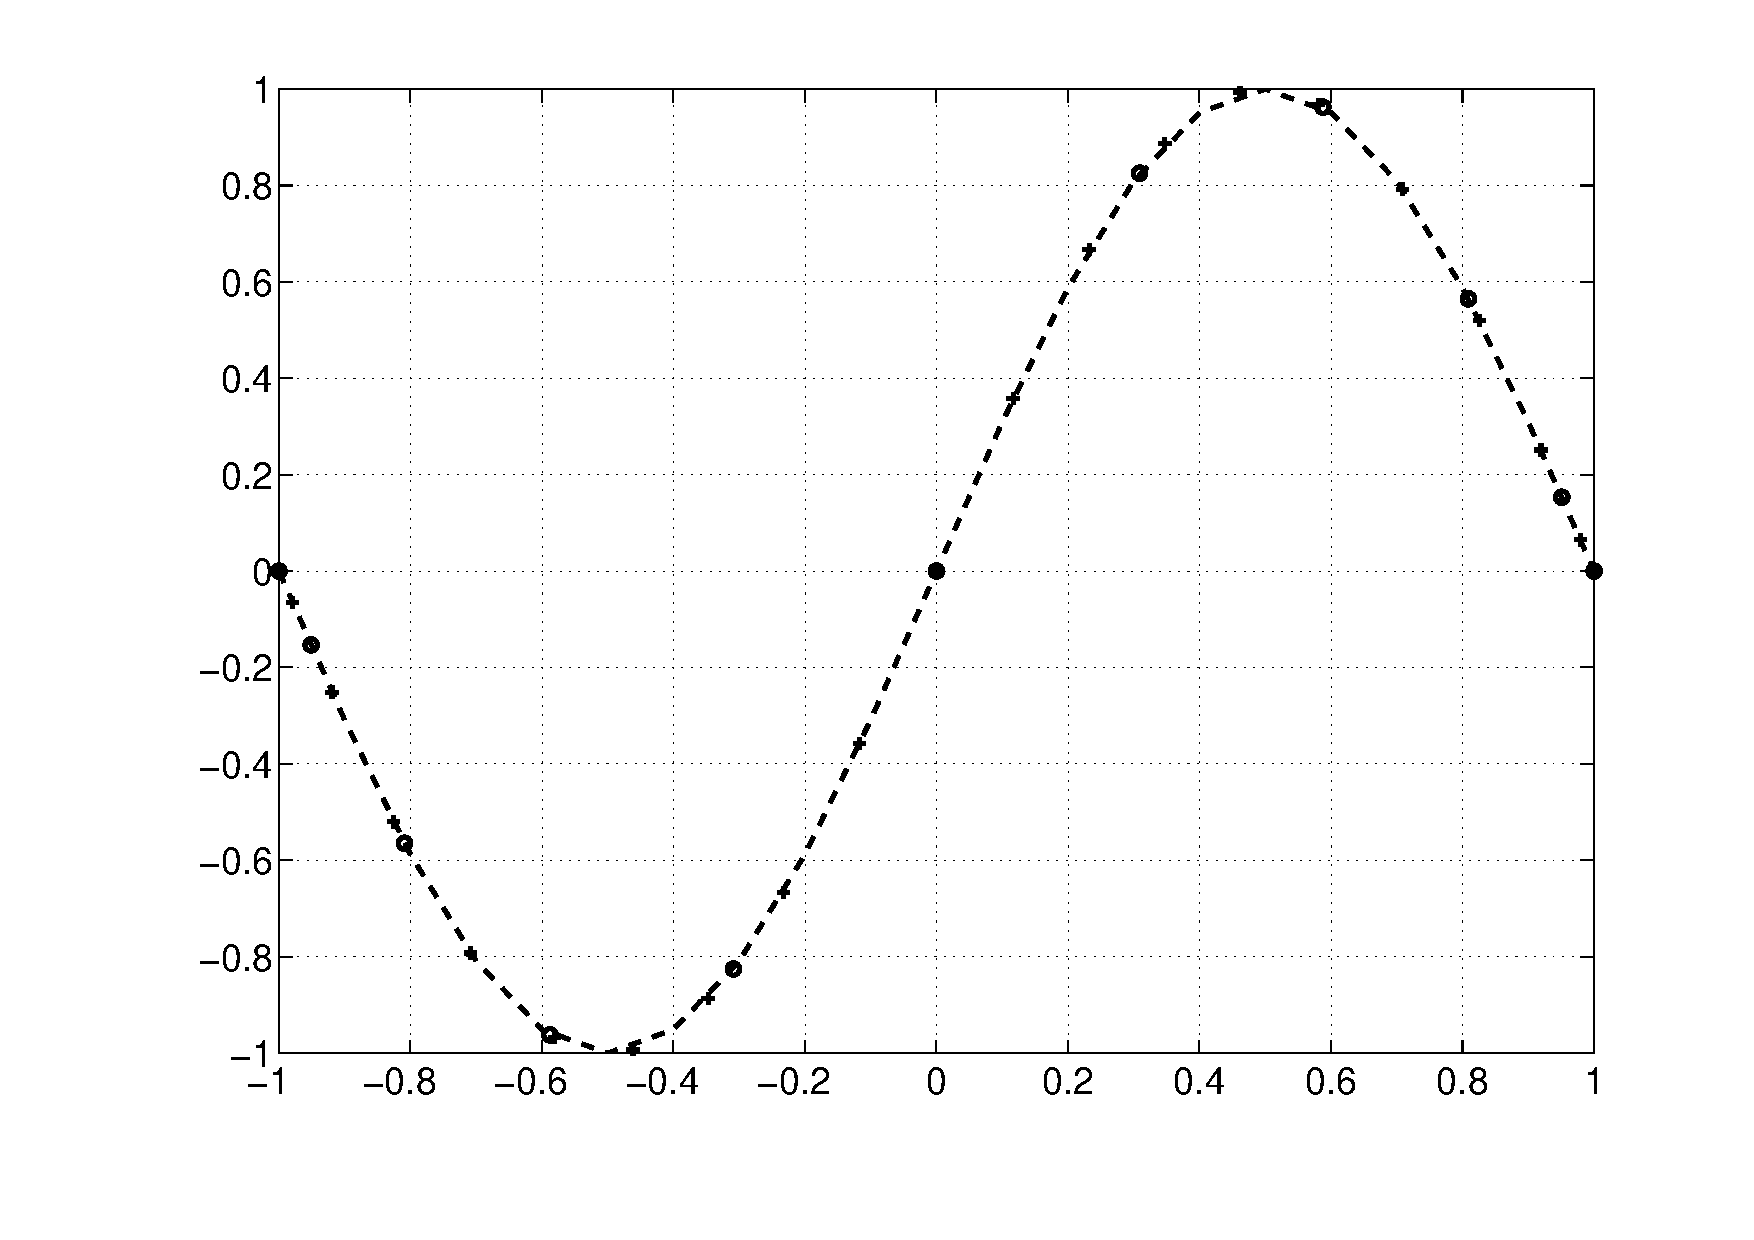
\includegraphics[scale=0.3, trim = 20mm 0mm 0mm 0mm, clip]{./Figures/1-HOFD/u_nonu.pdf}
\caption{$f(x)= sin(\pi x)$, non uniform mesh. }
\end{figure}

\columnbreak

\begin{figure}[H]
\centering
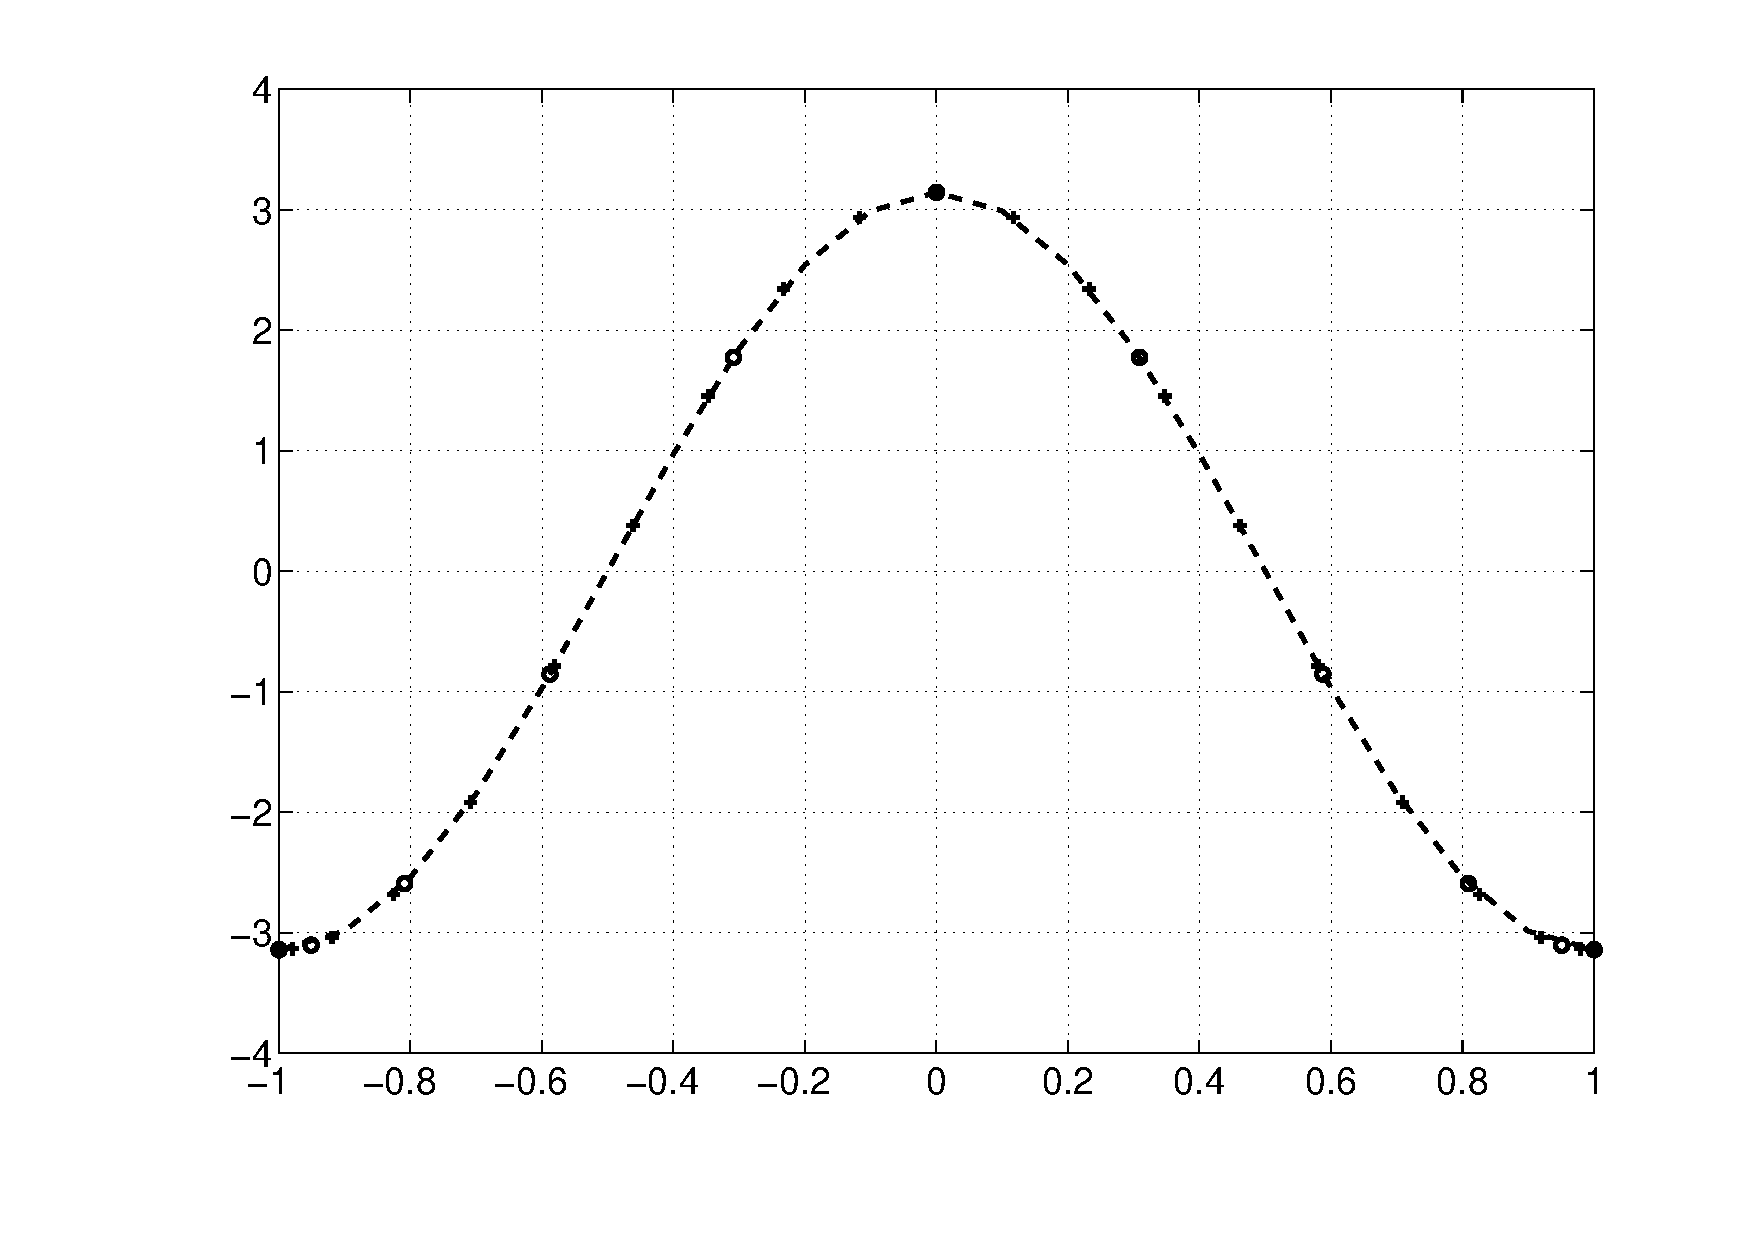
\includegraphics[scale=0.3, trim = 20mm 0mm 0mm 0mm, clip]{./Figures/1-HOFD/du_nonu.pdf}
\caption{$f'(x)$, non uniform mesh. }
\end{figure}

\columnbreak

\begin{figure}[H]
\centering
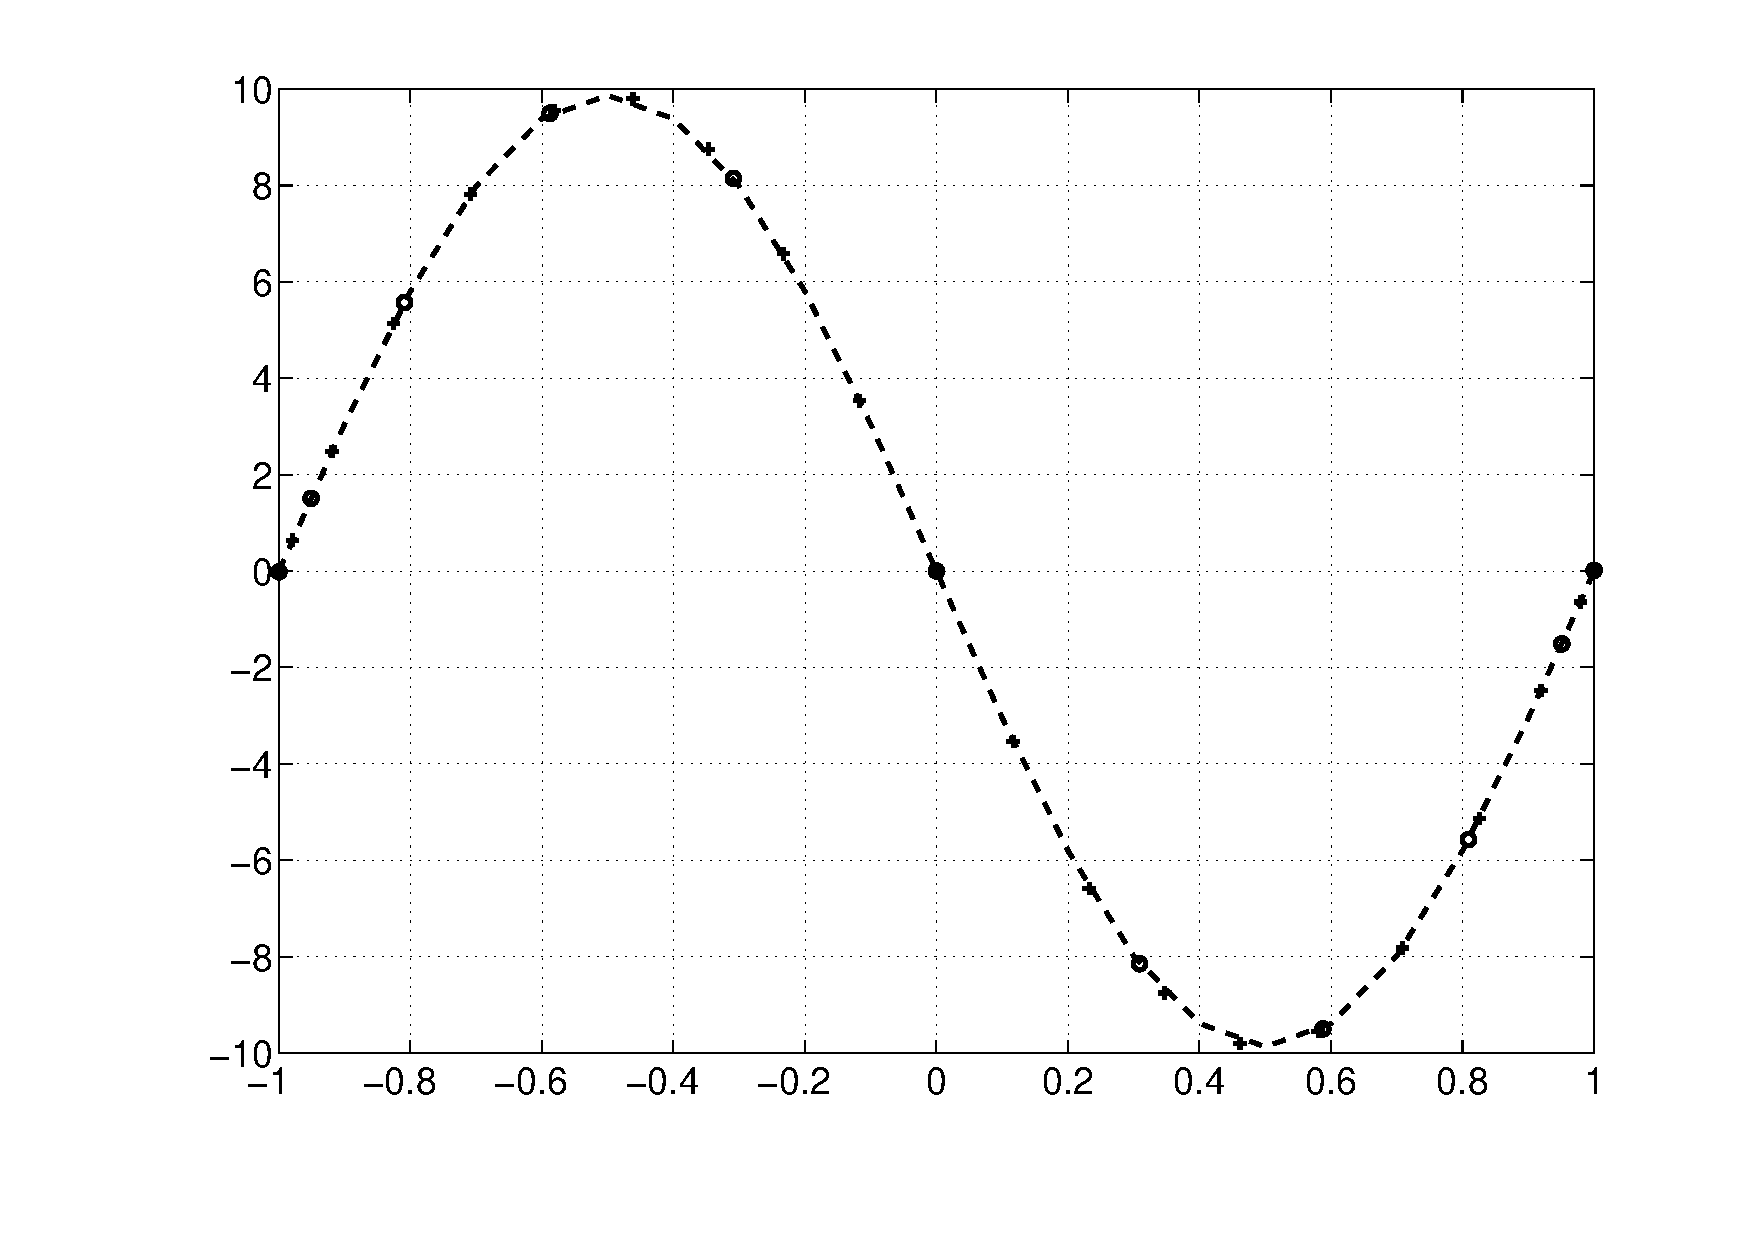
\includegraphics[scale=0.3, trim = 20mm 0mm 0mm 0mm, clip]{./Figures/1-HOFD/ddu_nonu.pdf}
\caption{$f''(x)$, nonuniform mesh. }
\end{figure}

\end{multicols}
\end{landscape}
\newpage

As we can see, the results are very accurate both using uniform and nonuniform
meshes. In the following figures the errors of the second derivative ($error=
u''_{exact}-u''_j$) are plotted:

\begin{multicols}{2}

\begin{figure}[H]
\centering
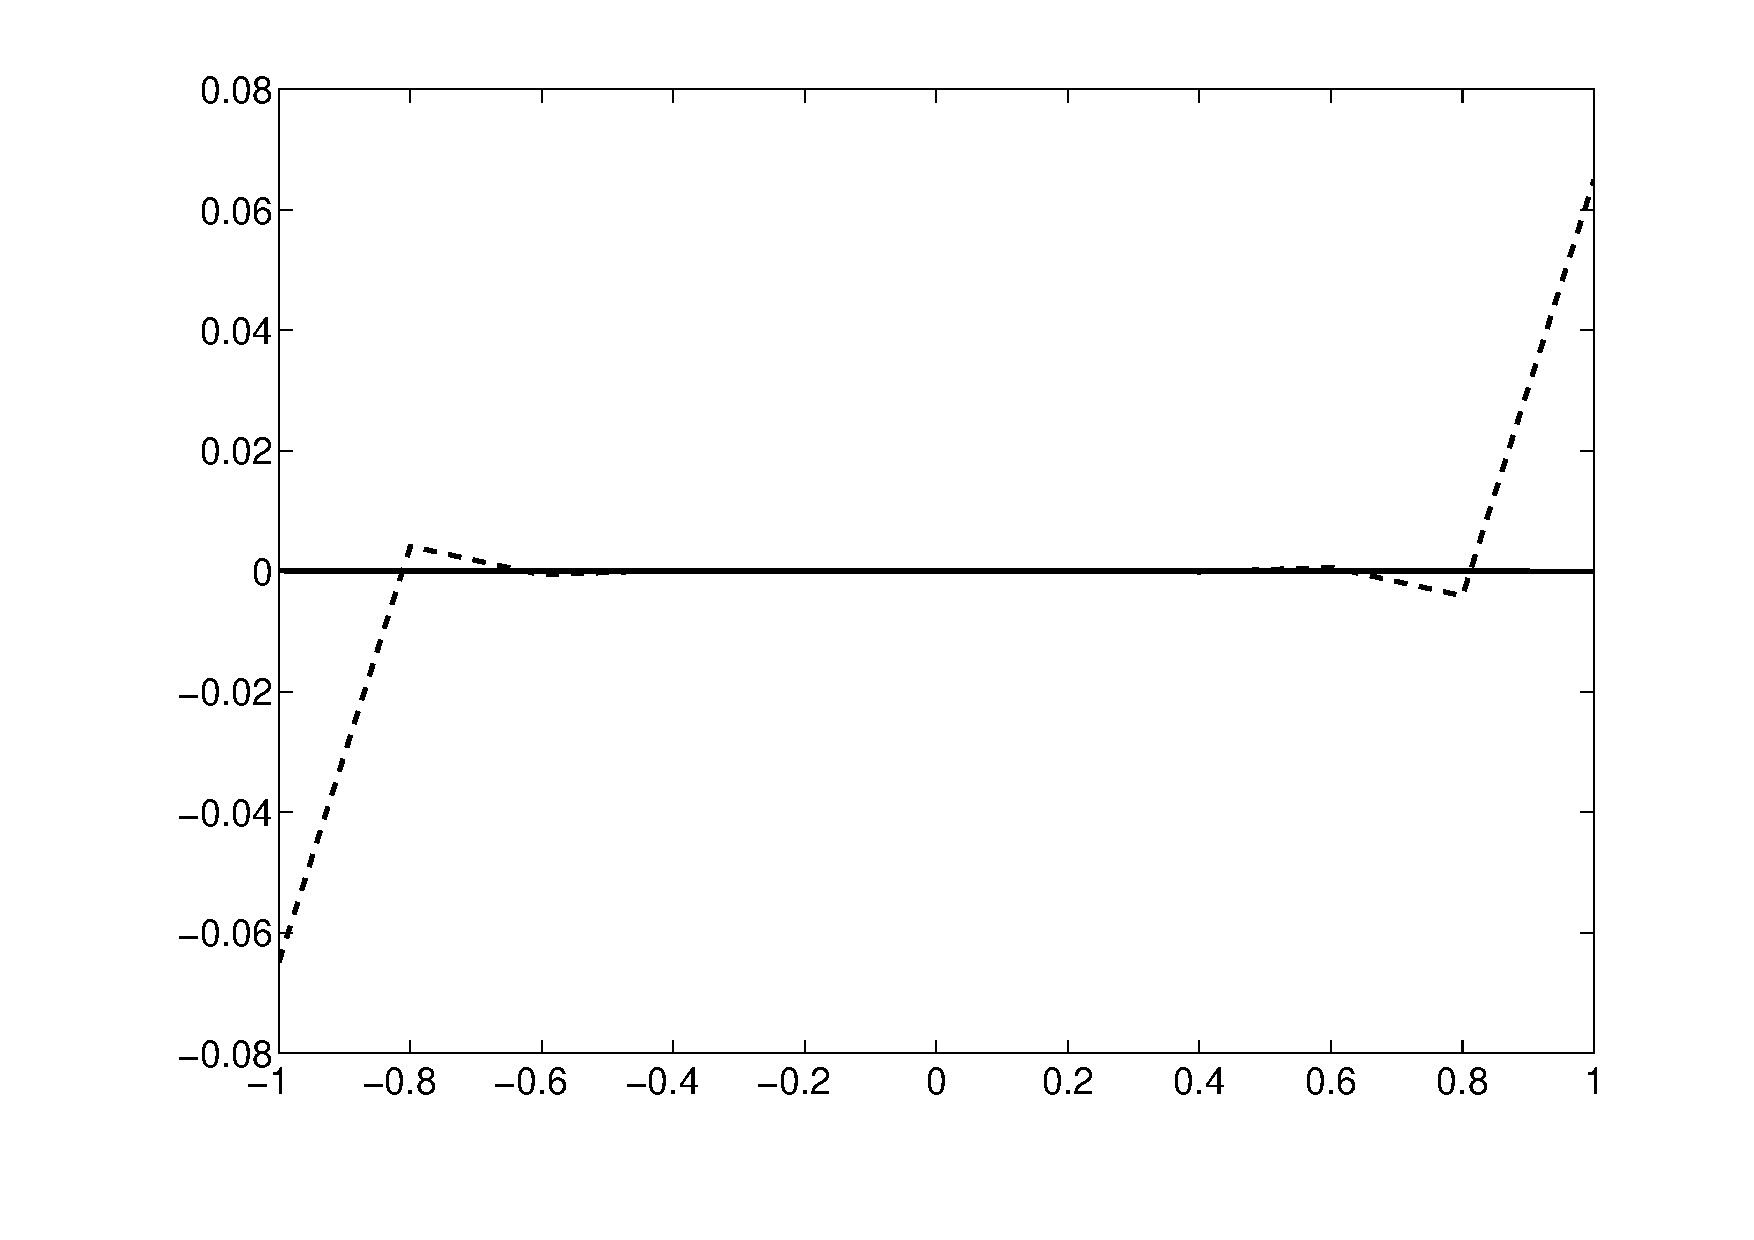
\includegraphics[scale=0.3, trim = 20mm 0mm 0mm 0mm, clip]
{./Figures/1-HOFD/error1.pdf}  \caption{Error of the uniform mesh using 10
(dashed) and 20 points (solid line).}
\end{figure}



\columnbreak

\begin{figure}[H]
\centering
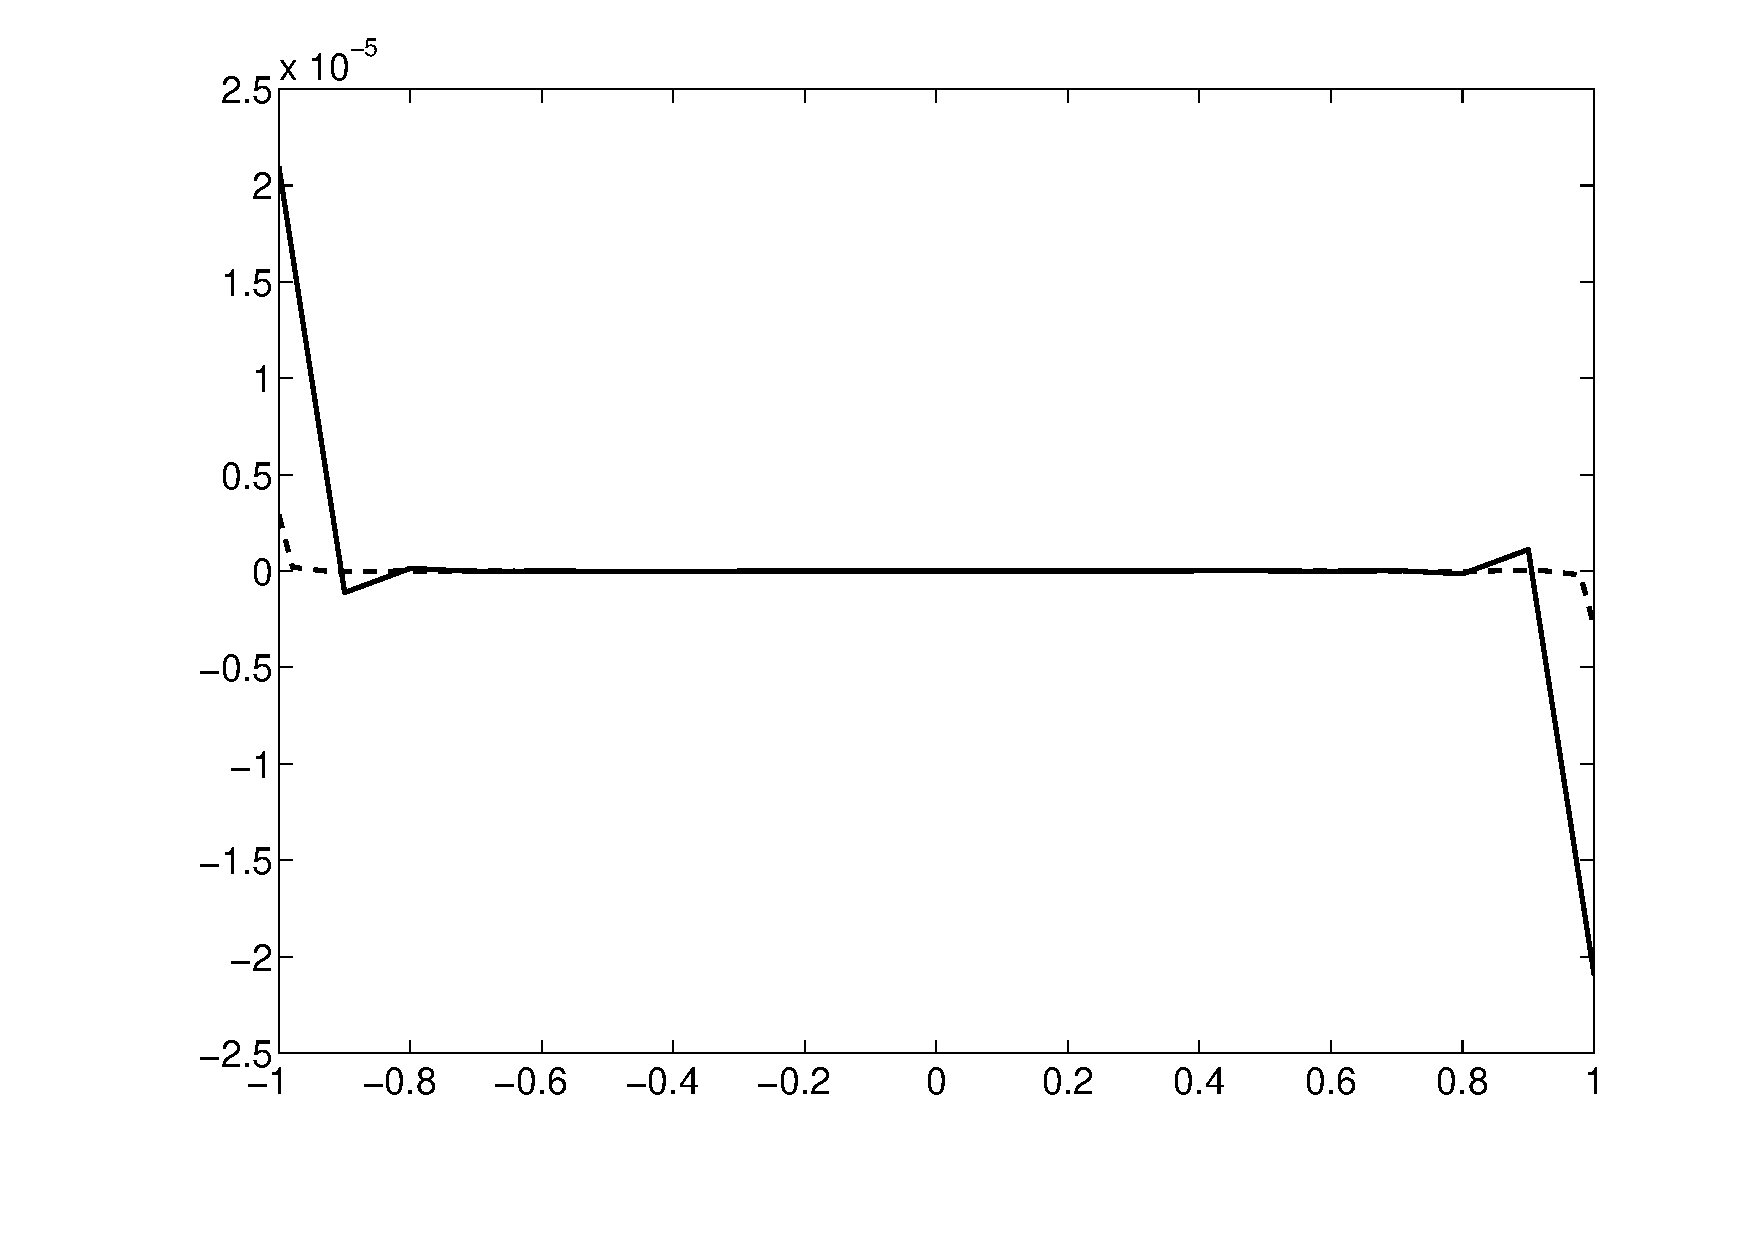
\includegraphics[scale=0.3, trim = 20mm 0mm 0mm 0mm, clip]{./Figures/1-HOFD/error2.pdf}
\caption{Error of the uniform mesh (solid line) and non uniform (dashed) using
20 points.}
\end{figure}

\end{multicols}

Besides the simplicity of this test case, we can see that the results obtained
are very good. Thus, we can extrapolate the functioning of this module to further applications. \\

\vspace{1cm}

In fact,  this program is able to calculate the derivatives of any
given 1D function $U=f(x)$ just changing the function definition line. The implications of this
simple method for such a complex procedure are many: 
\begin{itemize}
  \item The complexity is \textit{inside} the library. All that is seen from the
  API are some inputs and outputs arguments. 
  \item The syntax must be clear. In order to use the library, some rules must
  be regarded (in this case, the appropriate construction and arguments of the
  function \textit{Derivative}).
  \item The very same function is used for $x$ and $y$ derivatives, just
  changing the first input argument (\textit{Direction}).
\end{itemize}

The next example presents a 2D function. The idea is to show that the operations
are the same.\\

\newpage


\subsection{Laplacian of a function}
\label{laplacian}
% the \\ insures the section title is centered below the phrase: AppendixA
\begin{blueframed}
\begin{lstlisting}
program Laplacian

	use dislin
	use Finite_differences
	implicit none
	
	
  	integer, parameter :: N_x= 50, N_y= 50;!number of points
  	real ::  x(0:N_x), y(0:N_y)
	real:: U(0:N_x, 0:N_y)
	real:: Uxx(0:N_x, 0:N_y), Uyy(0:N_x, 0:N_y)
	real:: L(0:N_x, 0:N_y)
	integer :: Order = 20	!order of the interpolation
	integer :: i,j

	call Grid_Initialization( "uniform", "x", Order, x )
	call Grid_Initialization( "uniform", "y", Order, y )
	
	
	
	!function U=f(x,y)
	
	forall(i=0:N_x) U(i,:)=x(i)*x(i)+y*y ! an easy example
	
	 call Derivative( "x", 2, U, Uxx) 
	 call Derivative( "y", 2, U, Uyy) 

	 L=Uxx+Uyy
	 
	 ! Outputs (optional)
	  call scrmod('revers') 
	  call qplcon( L, N_x+1, N_y+1, 20);

end program
\end{lstlisting}
\end{blueframed}

The power of this library is clear with this example. Usually, computing the
\wk{Laplacian} of a function will involve a bunch of operations and a lot of
lines in our program. However, right now just one line is needed: $L=U_{xx}+U_{yy}$.\\

This procedure saves plenty of code lines with do-loops and complex
operations. The function assignment is written directly.\\

The next example continues with the higher complexity scale. The idea is to
prepare a program to perform the spatial discretization of the heat 1D
equation.\\

\newpage
\subsection{Heat equation (1D)}


We are going to deal with the following problem:

$$
\rho c_p \frac{\delta u}{\delta t}= k \frac{\delta^2 u}{\delta x^2};\;\;\;
+IC; \;\;\; +BC
$$

As we can see, this problem involves time and space. For now, we are just
interested in the \wk{spatial discretization}, so we are going to present the
operations for this purpose.\\

The idea is to transform the problem into something like: 

$$
\frac{\delta u}{\delta t}= \frac{k}{\rho c_p} \frac{\delta^2 u}{\delta
x^2};\;\Longrightarrow \frac{dU}{dt}= F(U,t)
$$

Also, the \wk{boundary conditions} must be discretized. Let's picture that the
boundary conditions are $u=T_0$ in $x=x_0$ and $\frac{\delta u}{\delta x}=0$ in $x=x_N$.\\

This is the example code for this application:

\begin{blueframed}
\begin{lstlisting}
subroutine heat_equation(t,U,F)

	real, intent(in) :: t
	real, intent(inout) :: U(:)
	real, intent(out) :: F(:)

	real :: alpha= 1., T0=1.
	real :: Uxx(0:Nx)
	
	integer:: Nx
	
	!Boundary conditions
	call Dirichlet ("x", 0, U, T0)
	call Newmann ("x", Nx, U, 0.0)

	!equation
	call Derivative("x",2,U,Uxx)
	
	F=alpha*Uxx
	
end subroutine
	
		
	
\end{lstlisting}
\end{blueframed}

Please, note that the program is not complete. There are some arguments that
have been supposed as knowns and some operations must be done before (meshing,
for example). Another module for the temporal discretization is needed in order to
solve the problem. However, the idea of this example is not to solve the
problem but to show the simplicity of the construction. The equation is written
the same way as it was when defining the problem:

$$
F(U,t)=\frac{k}{\rho c_p} \frac{\delta^2 u}{\delta
x^2} \Longrightarrow F=alpha*Uxx
$$






%%\end{document}
